\documentclass[journal, a4paper]{IEEEtran}
\usepackage[utf8]{inputenc}

\title{System Description}
% \author{sohanpatro2014 }
\date{December 2017}

\usepackage{natbib}
\usepackage{graphicx}

\usepackage{hyperref}
\hypersetup{
    colorlinks=true,
    linkcolor=blue,
    filecolor=magenta,      
    urlcolor=cyan,
}

\begin{document}

\maketitle

\section{Savitr front-end writeup}

\href{https://github.com/JaredHawkins/TweetGeoViz}\\

We started off by developing upon \href{https://github.com/JaredHawkins/TweetGeoViz}{TweetGeoViz}, which was developed in react and nodejs. 
However, due to its bulky nature, the system did not display any results when the database contained over 3 lakh tweets.\\

Owing to ease of control, we decided to port the complete system to Python. The current system, live on \href{http://savitr.herokuapp.com}{savitr.herokuapp.com}, works well at the same number of tweets. It has been built using flask and dash libraries.

\begin{figure}[h!]
\centering
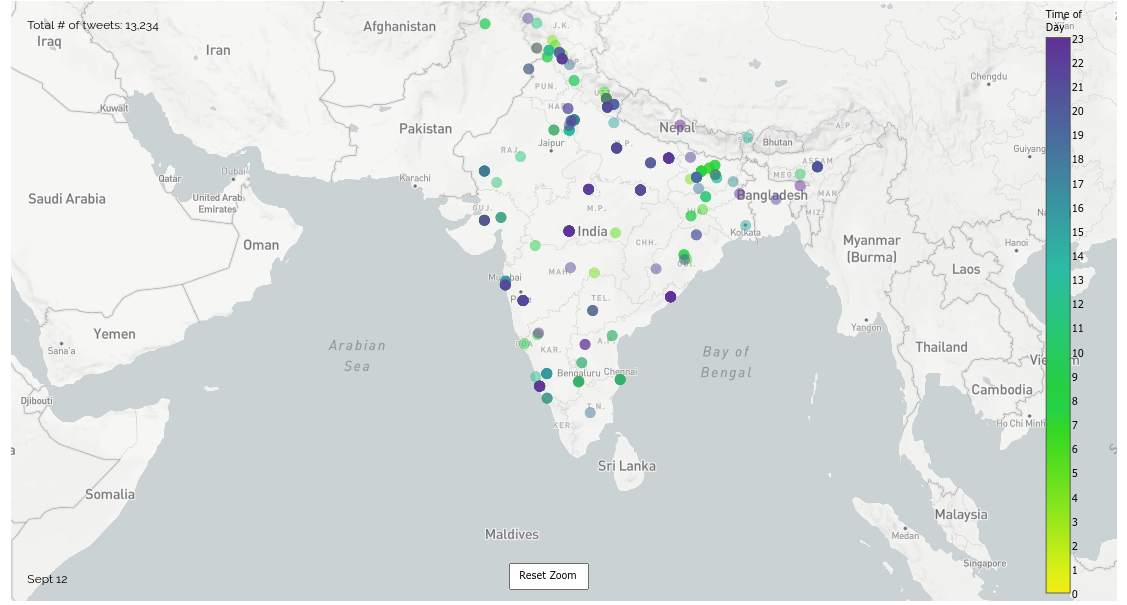
\includegraphics[width=\columnwidth]{map_general.png}
\caption{ Tweets visualized on India’s map}
\label{fig:map_general}
\end{figure}


\begin{figure}[h!]
\centering
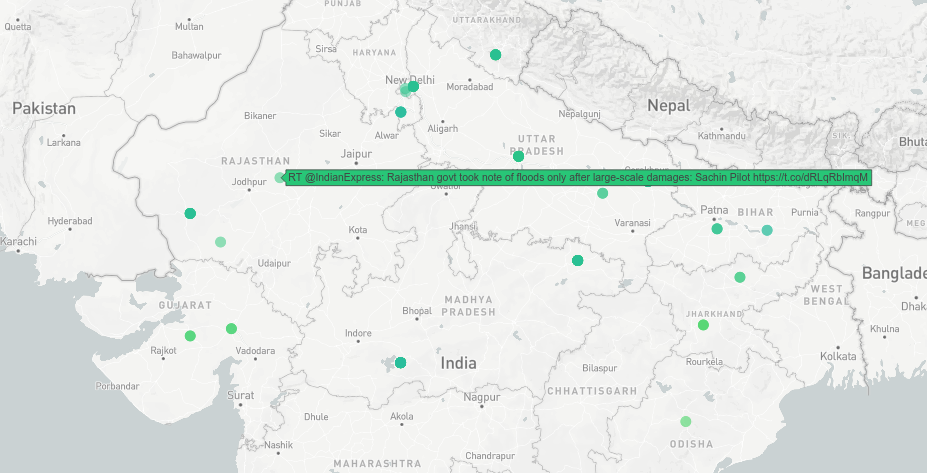
\includegraphics[width=\columnwidth]{map_hovertext.png}
\caption{Hovering over points reveal tweet text}
\label{fig:map_hovertext}
\end{figure}


The current system allows the user to search for tweets pertaining certain situations, like floods, dengue, etc. Hovering over a point reveals the tweet text. The possible situations were enlisted beforehand, but it will be possible to search for tweets containing any word.

\begin{figure}[h!]
\centering
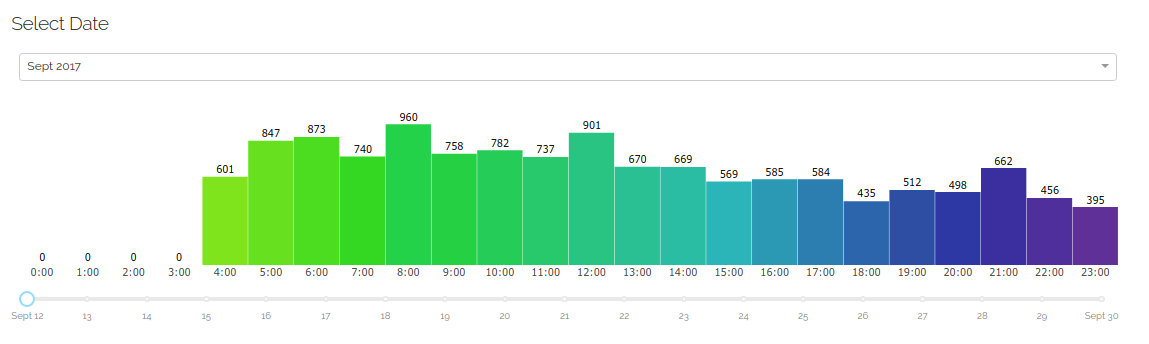
\includegraphics[width=\columnwidth]{bar_chart.png}
\caption{Tweets sorted by time of posting}
\label{fig:barchart}
\end{figure}


\begin{figure}[h!]
\centering
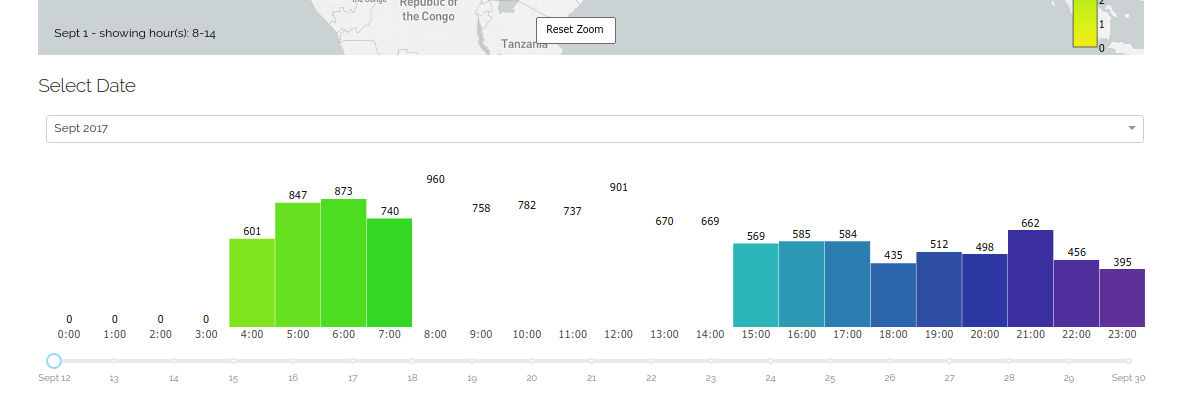
\includegraphics[width=\columnwidth]{bar_chart_specific.png}
\caption{Crosshair selection of time interval to visualise}
\label{fig:barchart_specific}
\end{figure}


\begin{figure}[h!]
\centering
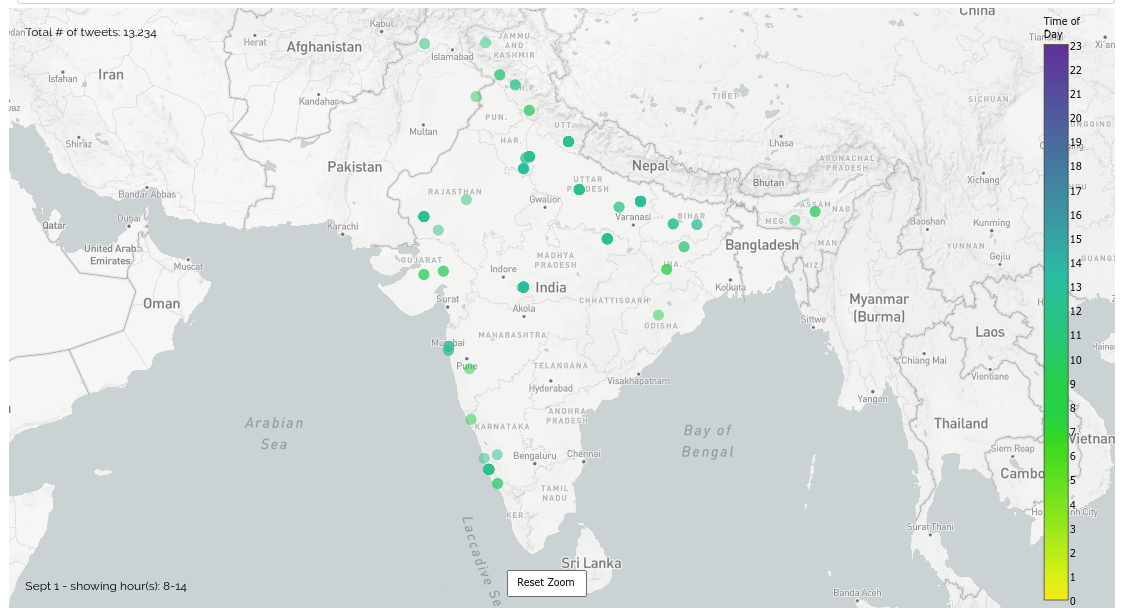
\includegraphics[width=\columnwidth]{map_specific.png}
\caption{ Tweets for certain time window displayed}
\label{fig:map_specific}
\end{figure}

\begin{figure}[h!]
\centering
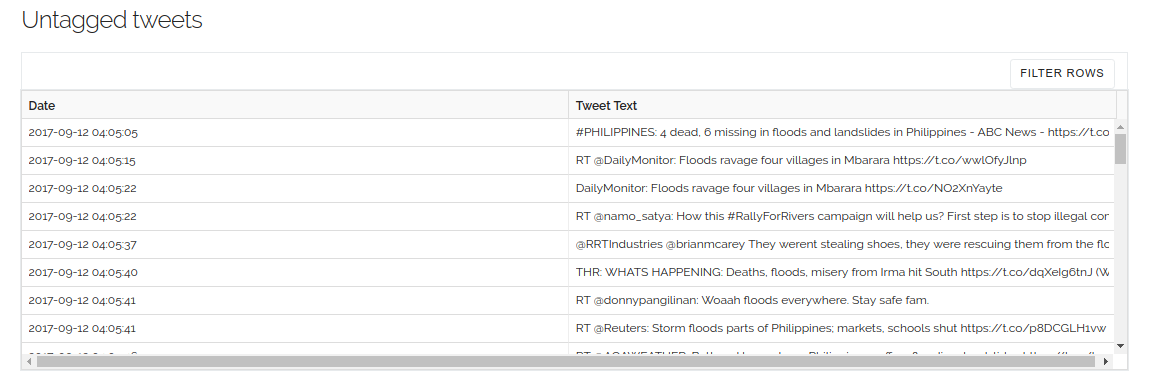
\includegraphics[width=\columnwidth]{untagged.png}
\caption{Untagged tweets displayed in tabular form at the bottom}
\label{fig:untagged}
\end{figure}

Untagged tweets are shown separately in tabular format at the very end. At any given instance, the user can see untagged tweets on a certain day. To reduce server strain, the user can only view data spanning 30 days, not more.

Further extensions to be added:
\begin{itemize}
    \item Currently, the data is being displayed from a static file. We will soon be shifting to a database support.
    \item The system will soon be able to visualise tweets spanning multiple days. Currently, the longest duration of tweets visualised in 1 day.
\end{itemize}

\end{document}
